\section{Fractional and stochastic preliminaries}
\subsection{Caputo derivative and long-memory interpretation}
\begin{definition}[Caputo derivative]
Let $u:[0,T]\to\R$ be absolutely continuous and let $0<\alpha<1$. The Caputo derivative of order $\alpha$ is defined by
\begin{equation}
\cD_t^{\alpha}u(t)=\frac{1}{\Gamma(1-\alpha)}\int_0^t\frac{u'(\tau)}{(t-\tau)^{\alpha}}\,d\tau.
\end{equation}
\end{definition}

The kernel $(t-\tau)^{-\alpha}$ induces a power-law memory. More recent changes contribute more strongly to the derivative than remote changes, but remote history never disappears entirely over a finite horizon. This property is fundamentally different from an integer-order derivative, which depends only on local variation. In logistics terms, the Caputo derivative provides a compact representation of persistence: earlier periods continue to affect the current state, though with decaying weight.

The order parameter $\alpha$ controls the effective memory depth. When $\alpha$ approaches one, the system behaves more like a classical first-order balance. When $\alpha$ is smaller, past states receive relatively more weight, and the operational system exhibits stronger path dependence. In the proposed transportation model, this interpretation can capture persistent congestion, delayed replenishment recovery, product-quality decay, or residual service distortion.

\begin{remark}
The use of the Caputo derivative is deliberate. In transportation and inventory applications, initial conditions are usually given in standard physical units such as initial stock, initial backlog, or initial service state. The Caputo operator accommodates such initial conditions more naturally than several alternative fractional derivatives.
\end{remark}

\subsection{Discrete-time approximation via the L1 scheme}
Because the optimization model is solved on a finite planning grid, the fractional state equation must be discretized. Let $t_n=n\Delta t$ for $n=0,1,\dots,N$, where $\Delta t=T/N$. For $0<\alpha<1$, the L1 approximation of the Caputo derivative at time $t_n$ is
\begin{equation}
\cD_t^{\alpha}u(t_n)\approx
\frac{1}{\Gamma(2-\alpha)\Delta t^{\alpha}}
\sum_{k=0}^{n-1}a_{n-k-1}(u_{k+1}-u_k),
\qquad a_r=(r+1)^{1-\alpha}-r^{1-\alpha}.
\end{equation}

The coefficients $a_r$ are positive and decreasing. This property is important because it preserves a natural interpretation of decaying memory. In the current optimization setting, the L1 discretization converts the continuous-time fractional differential equation into algebraic constraints linking all past states over the planning horizon. The resulting discretized model remains finite dimensional, but the memory effect creates dense temporal coupling.

To make the role of the coefficients explicit, define
\begin{equation}
\kappa_{n,r}(\alpha)=\frac{a_{n-r-1}}{\Gamma(2-\alpha)\Delta t^{\alpha}},\qquad r=0,1,\dots,n-1.
\end{equation}
Then each period-$n$ derivative depends on a weighted sum of all increments $u_{r+1}-u_r$. As a result, an imbalance corrected at one point in time still influences later periods through the remaining fractional memory.

\begin{figure}[H]
\centering
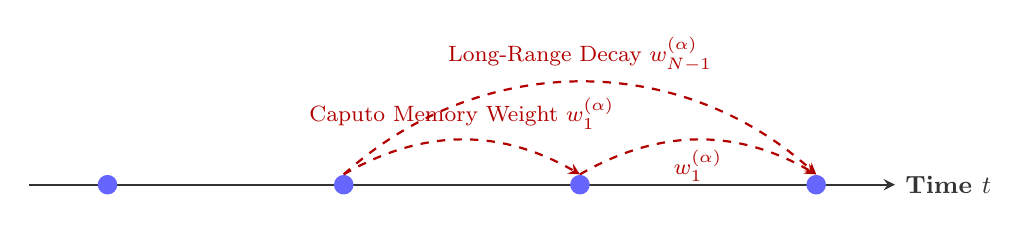
\begin{tikzpicture}[
    node distance=1.8cm,
    timeline/.style={->, >=stealth, thick, color=black!80},
    event/.style={circle, fill=blue!60, inner sep=2.5pt},
    label/.style={font=\small, align=center},
    memory/.style={->, >=stealth, dashed, thick, color=red!70!black}
]
    \draw[timeline] (0,0) to (11,0) node[right, font=\small\bfseries] {Time $t$};
    
    \node[event, label=below:{$t=0$\\Stage 1: $y_k, A$}] (t0) at (1,0) {};
    \node[event, label=below:{$t=1$\\Stage 2: $\omega \in \Omega$}] (t1) at (4,0) {};
    \node[event, label=below:{$t=2$\\Recourse $x_{ijt}^\omega, z_{jt}^\omega$}] (t2) at (7,0) {};
    \node[event, label=below:{$t=N$\\Horizon End}] (tn) at (10,0) {};
    
    \draw[memory] (t1.north) to[bend left=30] node[above, font=\footnotesize, color=red!70!black] {Caputo Memory Weight $w_1^{(\alpha)}$} (t2.north);
    \draw[memory] (t1.north) to[bend left=42] node[above, font=\footnotesize, color=red!70!black] {Long-Range Decay $w_{N-1}^{(\alpha)}$} (tn.north);
    \draw[memory] (t2.north) to[bend left=30] node[below, font=\footnotesize, color=red!70!black] {$w_1^{(\alpha)}$} (tn.north);
\end{tikzpicture}
\caption{Illustrative schematic of the two-stage stochastic information timeline and Caputo fractional memory feedback across decision epochs.}
\label{fig:timeline_schematic}
\end{figure}





\subsection{Stochastic demand representation}
Demand at customer $j$ is modeled in continuous time as a drift-diffusion process,
\begin{equation}
 dD_j(t)=\mu_j(t)\,dt+\sigma_j(t)\,dW_j(t),
\end{equation}
where $W_j$ is a standard Wiener process, $\mu_j(t)$ is the local drift, and $\sigma_j(t)$ is the volatility intensity. This representation is flexible enough to encode trend and variability while remaining consistent with scenario generation by Monte Carlo or lattice-based sampling.

For optimization, the continuous-time process is replaced by a finite scenario set $\Omega$. Each scenario $\omega\in\Omega$ specifies a full demand trajectory $\{d_{jt}^{\omega}:j\in J,t\in T\}$ together with probability $p_{\omega}$. The scenario approximation can be viewed as a sample-average representation of the demand law. In the numerical study, the scenario tree is synthetic and controlled, in an empirical deployment, the scenarios could be generated from historical residual resampling, a parametric stochastic model, or a forecast distribution.

\subsection{Risk measure: conditional value-at-risk}
Expected cost alone can understate operational exposure in highly adverse scenarios. To control tail behavior, the model uses conditional value-at-risk. Let $C^{\omega}$ denote the scenario cost and let $\beta\in(0,1)$ be the confidence level. The CVaR of the cost distribution at level $\beta$ can be expressed in optimization form as
\begin{equation}
\text{CVaR}_{\beta}(C)=\min_{\eta\in\R}\left\{\eta+\frac{1}{1-\beta}\sum_{\omega\in\Omega}p_{\omega}(C^{\omega}-\eta)_+\right\}.
\end{equation}
Introducing auxiliary variables $\xi_{\omega}\ge 0$ gives the linear constraints
\begin{equation}
\xi_{\omega}\ge C^{\omega}-\eta,\qquad \xi_{\omega}\ge 0,
\end{equation}
which can be embedded directly in the stochastic program. This representation is computationally convenient and managerially meaningful because it captures the average severity of the worst scenarios beyond the $\beta$-quantile.

\subsection{Carbon-trading balance}
Carbon regulation enters through an allowance-trading mechanism. Let $A$ denote the initial emissions allowance, $b^{\omega}$ the quantity purchased under scenario $\omega$, and $s^{\omega}$ the quantity sold. If total scenario emissions are $E^{\omega}$, the carbon-feasibility relation is
\begin{equation}
E^{\omega}\le A+b^{\omega}-s^{\omega}.
\end{equation}
When the buying price exceeds the selling price, the model naturally discourages simultaneous buying and selling. A formal statement of this property is proved later. In operational terms, the carbon-balance constraint turns emissions into a resource allocation problem rather than a passive accounting item.

